\documentclass[a4paper,twoside,12pt]{report}
\usepackage[utf8]{inputenc}
\usepackage[francais]{babel}
\usepackage[T1]{fontenc}
\usepackage{graphicx}
\usepackage{color}
\usepackage{url}
\usepackage{pdfpages}
\usepackage{amsmath}
\usepackage{amsfonts}
\usepackage{amssymb}
\usepackage{caption}
\usepackage{wrapfig}
\usepackage[left=2cm, right=2cm, top=2.75cm, bottom=2cm]{geometry}
\usepackage{graphicx}
\usepackage{fancyhdr}
\usepackage[pdftex]{hyperref}
\usepackage{eurosym}
\usepackage{float}
\usepackage{pdfpages}
\usepackage{insa}
\usepackage{todonotes}
\usepackage{listings}

\lstdefinelanguage{scala}{
  morekeywords={abstract,case,catch,class,def,%
  do,else,extends,false,final,finally,%
  for,if,implicit,import,match,mixin,%
  new,null,object,override,package,%
  private,protected,requires,return,sealed,%
  super,this,throw,trait,true,try,%
  type,val,var,while,with,yield},
  otherkeywords={=>,<-,<\%,<:,>:,\#,@},
  sensitive=true,
  morecomment=[l]{//},
  morecomment=[n]{/*}{*/},
  morestring=[b]",
  morestring=[b]',
  morestring=[b]"""
}

\definecolor{dkgreen}{rgb}{0,0.6,0}
\definecolor{gray}{rgb}{0.5,0.5,0.5}
\definecolor{mauve}{rgb}{0.58,0,0.82}

% Default settings for code listings
\lstset{frame=tb,
  language=scala,
  aboveskip=3mm,
  belowskip=3mm,
  showstringspaces=false,
  columns=flexible,
  basicstyle={\small\ttfamily},
  numbers=none,
  numberstyle=\tiny\color{gray},
  keywordstyle=\color{blue},
  commentstyle=\color{dkgreen},
  stringstyle=\color{mauve},
  frame=single,
  breaklines=true,
  breakatwhitespace=true
  tabsize=3,
  numbers=left,
  numberstyle=\tiny\color{gray}
}

\hypersetup{
	unicode=false,
	colorlinks=true,
	citecolor=black,
	filecolor=black,
	linkcolor=black,
	urlcolor=black
}

\newcommand{\excilys}{Excilys}
\newcommand{\excilysGroup}{Groupe \excilys{}}
\newcommand{\ebi}{eBusiness Information}
\newcommand{\capico}{Capico}

\begin{document}

\pageDeGarde[cover.pdf]{Stage ingénieur}{Évolution du système d'information du \excilysGroup}{Tuteur école :\\Stéphane CANU\\Tuteur entreprise :\\François-Pierre CHALOPIN}{Grégory COUTANT}

\pagestyle{fancyplain}
\fancyhf{}

\pageINSA[twoside]

\setcounter{page}{1}

\chapter*{Remerciements}
\addcontentsline{toc}{chapter}{Remerciements}

Je souhaite tout d'abord remercier M. Chalopin, M. Reby et M. Duvoid pour m'avoir accueilli chaleureusement au sein de leur société.\\

Je voudrais également remercier M. Landelle et M. De Domenico pour leur suivi, leur partage de connaissances et les nombreux conseils qu'ils ont pu me prodiguer ainsi que pour leur patience envers les stagiaires.\\

Je souhaite aussi remercier l'équipe administrative qui m'a accompagnée tout au long de ce stage, et plus particulièrement Mlle Sergio pour sa gentillesse lors des phases de séléction des stagiaires.\\

Finalement, j'aimerais remercier les consultants, les commerciaux et les autres stagiaires que j'ai pu cotoyer pendant mon stage pour leurs compétences et la bonne humeur qu'ils ont pu véhiculer.

\newpage
\pdfbookmark[0]{Table des matières}{toc}
\tableofcontents

\chapter*{Introduction}
\addcontentsline{toc}{chapter}{Introduction}

Le présent rapport a pour but de montrer le déroulement et analyser le travail effectué lors de mon stage ingénieur arrivant à la fin de ma formation dans le département Architecture des Systèmes d'Informations à l'Institut National des Sciences Appliquées.\\

Ce stage d'une durée de 6 mois s'est déroulé au sein d'\ebi{}, une SSII située à Cachan spécialisée dans les technologies Java/JEE. Ce stage s'est globalement découpé en deux parties : une formation sur les technologies Java/JEE et les frameworks associés et la participation aux développements de projets internes au \excilysGroup{}.


\chapter{Présentation de l'entreprise}

\ebi{} est une société de services basée en région parisienne et appartient au \excilysGroup{} \cite{excilys}.

\section{Le \excilysGroup{}}

\excilys{} est un groupe regroupant sept sociétés de services (Adlys, Altendis, \ebi{}, Edvance, Equitalis, SS2J et Visual3X) spécialisé dans les technologies Java/JEE. Ce groupe est né du développement d'\ebi{}.

\subsection{Historique du groupe}

L'histoire de la société commence en 2000 avec la création d'\ebi{}. Cette entreprise avait pour vocation de répondre à des problématiques pointues dans le cadre de développement Java/JEE, notamment dû au fait que les grands comptes manquaient d'expertises sur ce domaine.
\ebi{} s'est placée sur cette niche de l'expertise technique en Java/JEE, dans le secteur de l'assurance puis graduellement dans d'autres secteurs d’activités (Santé, Banque, Sécurité, Fret…).\\

En 2002, l’entreprise a décidé de refondre son organisation interne, que ce soit au niveau de la gestion des rémunérations, la gestion des carrières ou le recrutement. Ce remaniement profond a donné naissance à la charte \excilys{} (cf. annexe~\ref{ann:charte}).
Cette charte définit des règles que la société s'impose envers ses clients et ses consultants. Elle définit un modèle pour la prestation de service : le Service Équitable.\\

Les résultats probants de cette démarche ont poussé l'entreprise à se développer en proposant ce modèle à d'autres sociétés de services voulant se spécialiser dans l'excellence technique. \excilys{} est né.

\subsection{La société \ebi{}}

\ebi{} se concentre toujours dans l'expertise technique dans le domaine Java/JEE en proposant conseils et développements à ses clients.
La société intervient également en tant que sous-traitant de grandes sociétés de services pour définir l'architecture de leur projet tout en encadrant leurs équipes.
La société, étant experte sur un domaine, s'est logiquement dirigée vers le coaching et l'organisation de formations.\\

Elle propose en effet des cycles de formation complets (Java Academy), des audits d'infrastructures, l'implantation de solution Open Source ou encore de l'assistance à maîtrise d'ouvrage dans le cadre d'un développement d'applications JEE.\\

\begin{figure}[H]
	\centering
	
\includegraphics[width=\linewidth]{images/diag_metier.pdf}
	\caption{Les 4 métiers}
\end{figure}


Compte tenu des bons résultats de l'entreprise, elle dispose désormais de nombreux clients, dans de multiples secteurs d'activités.\\

\begin{figure}[H]
	\centering
	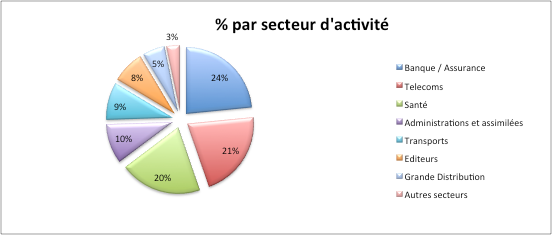
\includegraphics[width=\linewidth]{images/pie_ca.pdf}
	\caption{Répartition du chiffre d'affaires par secteur d'activité}
\end{figure}

En 2009, \ebi{} a décidé d'élargir son pôle de compétences en investissant notamment sur les plateformes mobiles Android, puis sur des plateformes iOS (iPhone) en 2010. Elle a aussi décidé de monter en compétences dans un secteur porteur : le cloud, notamment AppEngine (Google) et Amazon EC2 et S3.\\

Au niveau économique, \ebi{}  est une SARL ne disposant d'aucun investisseur financier externe. Son chiffre d'affaires est en constante augmentation jusqu'en 2008, puis en diminution en 2009 : conséquence de la crise financière. Il retrouve finalement un niveau équivalent à 2008 en 2010 avec un chiffre d'affaires hors taxe de 7.4 M\euro{}.\\

\begin{figure}[H]
	\centering
	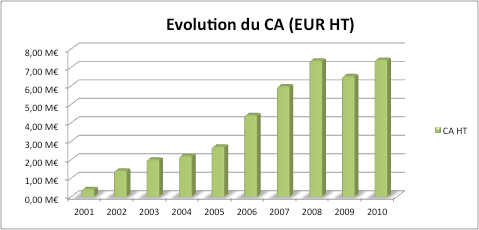
\includegraphics[width=\linewidth]{images/diag_ca.pdf}
	\caption{Évolution du chiffre d'affaires}
\end{figure}

\subsection{Les autres entités du groupe}

En plus d'\ebi{}, le groupe compte six autres sociétés respectant la charte \excilys{} dans des domaines similaires :

\begin{description}
	\item [Altendis] 
	Spécialisée dans le développement Java/JEE avec des profils moins expérimentés que ceux d'\ebi{}, la société offre des prestations essentiellement dans des projets de développements. Cette société emploie directement les stagiaires en fin de stage.
	
	\item [SS2J] 
	Spécialisée autour de la conduite de projets, la société offre des prestations dans le domaine du coaching, la gestion de projets en suivant les méthodes agiles.
	
	\item [Edvance] 
	La société est spécialisée dans les solutions autour de la technologie RFID (\textit{Radio Frequency IDentifier}). La société est partenaire de STMicroElectronics et offre parmi ses solutions, un système complet de gestion des accès à un bâtiment par contrôle RFID/JEE des personnes.
	
	\item [Equitalis]
	L'entreprise est située à Bordeaux. Equitalis propose des prestations similaires à \ebi{} (architecture JEE, gestion de projets Agile, formation et coaching). Elle est la première société basée en province respectant la charte \excilys{}.
	
	\item [Adlys]
	Adlys est une société de conseil, d'ingénierie et de formation, spécialisée dans les infrastructures Java/JEE qui a notamment apporté son expérience dans le domaine du coaching et de la formation aux autres sociétés du groupe.
	
	\item [Visual3X] 
	Visual3X est la société spécialisée dans la mise en place de clients riches et d'interface Web 2.0 et propose du conseil, de la formation ou du développement. 
\end{description}

\section{L'organisation de l'entreprise}

\ebi{} étant détenue intégralement par ses dirigeants, l'entreprise reste maître de son évolution et de son fonctionnement, en restant régie par la charte \excilys{}.

\subsection{Le service équitable - La charte \excilys{}}

La charte \excilys{} est une action assez unique en son genre dont le but est de prôner certaines valeurs pour assurer une meilleure implication des consultants chez leurs clients. Ceci passe par un salaire du consultant proportionnel à la facturation cliente et des consultants adaptés à la mission.

\begin{figure}[H]
	\centering
	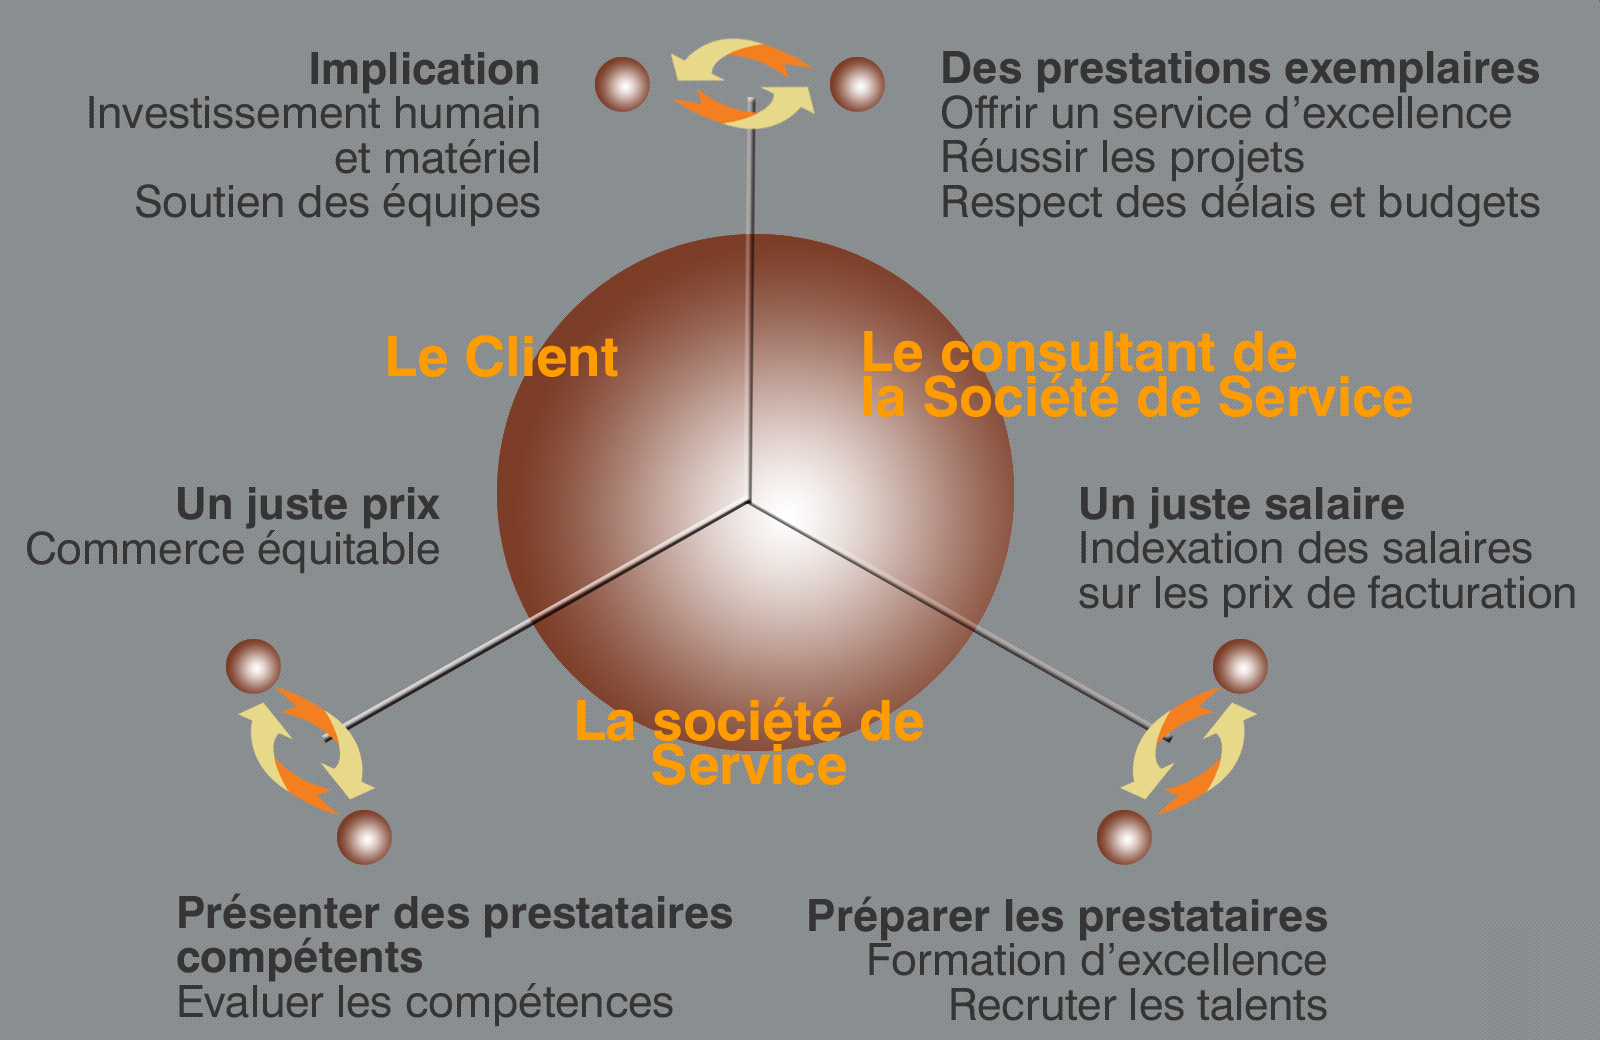
\includegraphics[width=\linewidth]{images/diag_equi.pdf}
	\caption{Le service équitable}
\end{figure}

Pour préparer les consultants, \ebi{} s’appuie sur des formations et le partage de connaissances qui est un des aspects les plus importants pour \excilys{} car il permet une montée en compétence rapide de ses consultants. Pour mener à bien cette action, un système de capitalisation de compétences, \capico{} \cite{capico}, développé en interne, a été mis en place.

\subsection{Le système d'information du groupe}

Le système d'information du groupe \excilys{}, est composé de différents modules : 

\begin{itemize}
	\item Les modules fonctionnels 
	\item Les modules techniques
	\item La gestion des droits\\
\end{itemize}

Les modules fonctionnels correspondent à tous les outils permettant de gérer la plupart des problématiques pour l'entreprise, c’est-à-dire tous les aspects de gestion commerciale mais également la gestion des compétences et des connaissances ou encore les aspects communications (Mail ,site internet , blog, forum,\ldots). Les aspects administratifs sont également gérés via une application développée en interne, Maestro.\\

Les modules techniques servent de support aux modules fonctionnels.
Finalement, la gestion des droits permet de gérer, via le module Security, les accès aux différents modules.
A terme, l'ensemble des services sera géré via un ESB(\textit{Entreprise Service Bus}).
Les stages effectués chez \ebi{} se déroule généralement sur une partie du système d'information, notamment dans les modules fonctionnels.
Mon stage s'est donc porté sur l'application d'e-coaching et d'e-learning du groupe : \capico{}.

\begin{figure}[H]
	\centering
	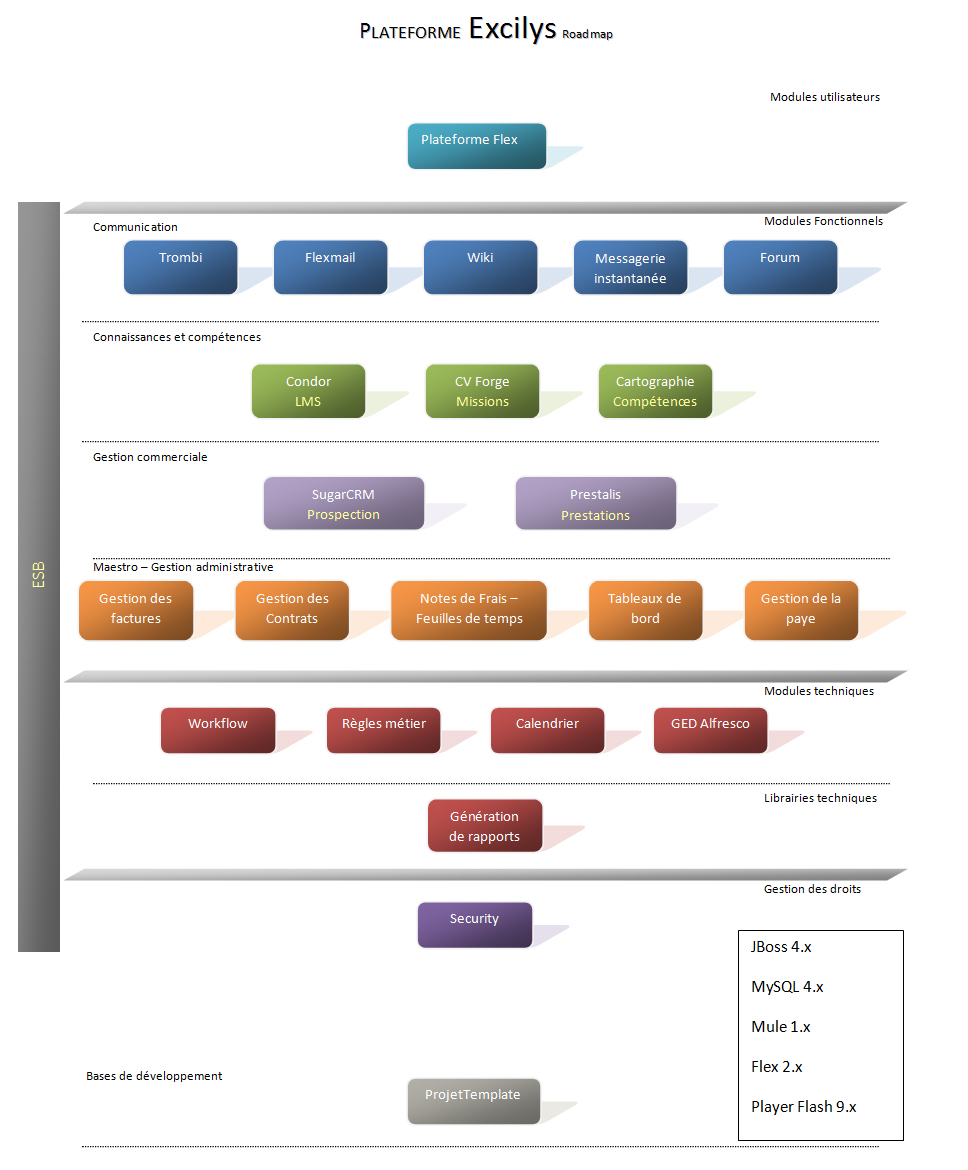
\includegraphics[width=\linewidth]{images/diag_si.pdf}
	\caption{Système d'information du groupe \excilys{}}
\end{figure}


\chapter{Présentation du stage}

\section{Sujet du stage}

Le sujet du stage, tel qu'il est défini dans la convention :\\

\emph{Évolutions de systèmes d'informations Java/JEE : Le stagiaire participera au développement de notre système d'information ou à celui de l'un de nos clients dans les technologies Java/JEE. Il sera d'abord formé à l'utilisation de différents outils et frameworks, puis les mettra en \oe{}uvre dans le cadre du projet auquel il participera sous la conduite d'un architecte logiciel.}\\

Le \excilysGroup{} recrutant exclusivement après un stage ingénieur effectué au sein d'\ebi{}, les stages proposés contiennent une importante partie de formation. Cette formation permet de garantir son engagement d'excellence technique auprès de ses clients. Une première partie du stage, durant deux mois, est donc consacré à la formation. Pendant la seconde partie, les stagiaires sont amenés à participer à des projets internes.

\section{La formation}

La première partie de mon stage a donc été une période de formation durant environ deux mois. Durant cette période, les stagiaires utilisent la plateforme d'e-learning Capico, dans laquelle un grand nombre de technologies et de frameworks Java/JEE sont abordés sous forme de cours, de QCM et d'exercices pour la mise en pratique des technologies étudiées.\\

Cette partie de formation sur Capico, d'une duré d'un mois, m'a permis d'étudier en profondeur le langage Java, la plateforme JavaEE et de nombreux outils et frameworks utilisés dans le monde de l'entreprise tels que Spring, Hibernate, Maven, Subversion, Log4J, \dots{} De plus, des méthodes de gestion de projets Agiles ont été abordées telles que Scrum et l'eXtreme Programming (XP).\\

Pendant le mois suivant, les connaissances fraîchement apprises sont mises en pratique dans un mini-projet consistant en la réalisation d'une application web d'e-banking. Ce mini-projet est réalisé en groupe de plusieurs stagiaires sous la tutelle de Stéphane LANDELLE, directeur technique d'\ebi{}. Il intervient à la fois comme client de notre application, et comme référent technique.

Dans le but d'assurer aux clients le bon niveau technique de ses consultant, \ebi{} demande à ses stagiaires de passer la certification Oracle Certified Java Programmer. J'ai donc en parallèle de la formation préparé celle-ci et réussi à obtenir le score de 91\%, 61\% étant suffisant pour l'obtenir. 

\section{Gatling}

Après cette phase de formation, j'ai été amené à travailler sur le projet Gatling pendant une durée de quatre mois. Gatling est une application permettant d'effectuer des tests de charge sur des applications web. Elle est principalement développée par Stéphane LANDELLE et est open source dans sa majeure partie. Cette application est notamment utilisée lors d'audits techniques d'applications réalisés par \ebi{}.\\

Mon travail en collaboration avec deux autres stagiaires a consisté à réalisé un état de l'art de plusieurs technologies pour évaluer la faisabilité de nouvelles fonctionnalités à ajouter à Gatling. Puis de développer certaines d'entre elles. Ces fonctionnalités sont :

\begin{itemize}
	\item Récupération de métriques du serveur contenant l'application en test pour les mettre en relation avec les métriques du côté client, générées par Gatling,
	\item Exposition en temps réel des métriques mesurées par Gatling vers un système tiers de monitoring temps réel,
	\item Amélioration du système de génération de rapport pour pouvoir générer des rapports lors de tests produisant une grande quantité de données brutes (~ 10 Go).
	\item Réalisation d'un plugin Jenkins pour suivre une simulation Gatling au sein d'un projet et ainsi de pouvoir déterminer des conditions d'échec ou d'instabilité du build en fonction des résultats des tests de charge et d'afficher l'évolution des performances.\\
\end{itemize}

En parallèle, je me suis formé sur les technologies utilisées par Gatling que sont le langage de programmation multi-paradigme Scala ainsi que le framework Akka.

\chapter{Travail effectué}

Mon stage s'est déroulé en trois phases :

\begin{itemize}
	\item La formation pure d'une durée de 5 semaines sur la plateforme d'e-learning Capico,
	\item Le mini-projet d'e-banking pendant 5 semaines, pour la mise en pratique des connaissances fraîchement apprises,
	\item La recherche et le développement de fonctionnalités dans Gatling pendant 4 mois.\\
\end{itemize}

Je vais maintenant détailler le travail effectué lors de chacune d'entre elles.

\section{La formation}

\subsection{Contenu}

La formation dispensée a pour but principal de mettre tous les stagiaires au même niveau sur les principales technologies Java/JEE utilisées dans le monde de l'entreprise.\\

Nous avons ainsi abordé les sujets suivants :

\begin{itemize}
	\item eXtreme Programming
	\item UML
	\item Subversion
	\item Maven 2
	\item Java 5
	\item Log4J
	\item JDBC
	\item JUnit 3 et 4
	\item JEE
	\item Hibernate 3
	\item Spring 2.5\\
\end{itemize}

Les technologies abordées sont pour la plupart survolées et certaines sont dépassées, bien que toujours grandement utilisées. La formation sert ainsi de socle pour une auto-formation plus en détail de ces même technologies ou bien de leurs successeurs. Cette auto-formation est une composante indispensable du métier de consultant puisqu'elle permet de rester à un certain niveau d'expertise, de pouvoir anticiper les évolutions techniques et, éventuellement, de pouvoir être force de proposition sur la direction d'un projet.

\subsection{Déroulement}

L'ensemble de la formation se fait via la plateforme d'e-learning développée par \excilys{}, à savoir Capico \cite{capico}. Elle consiste en une suite de cours magistraux éventuellement sonorisés pour une meilleure compréhension. Ces cours sont accompagnés de QCM pour vérifier que les connaissances ont bien été assimilées ainsi que d'exercices pour la mise en pratique.

\begin{figure}[H]
	\centering
	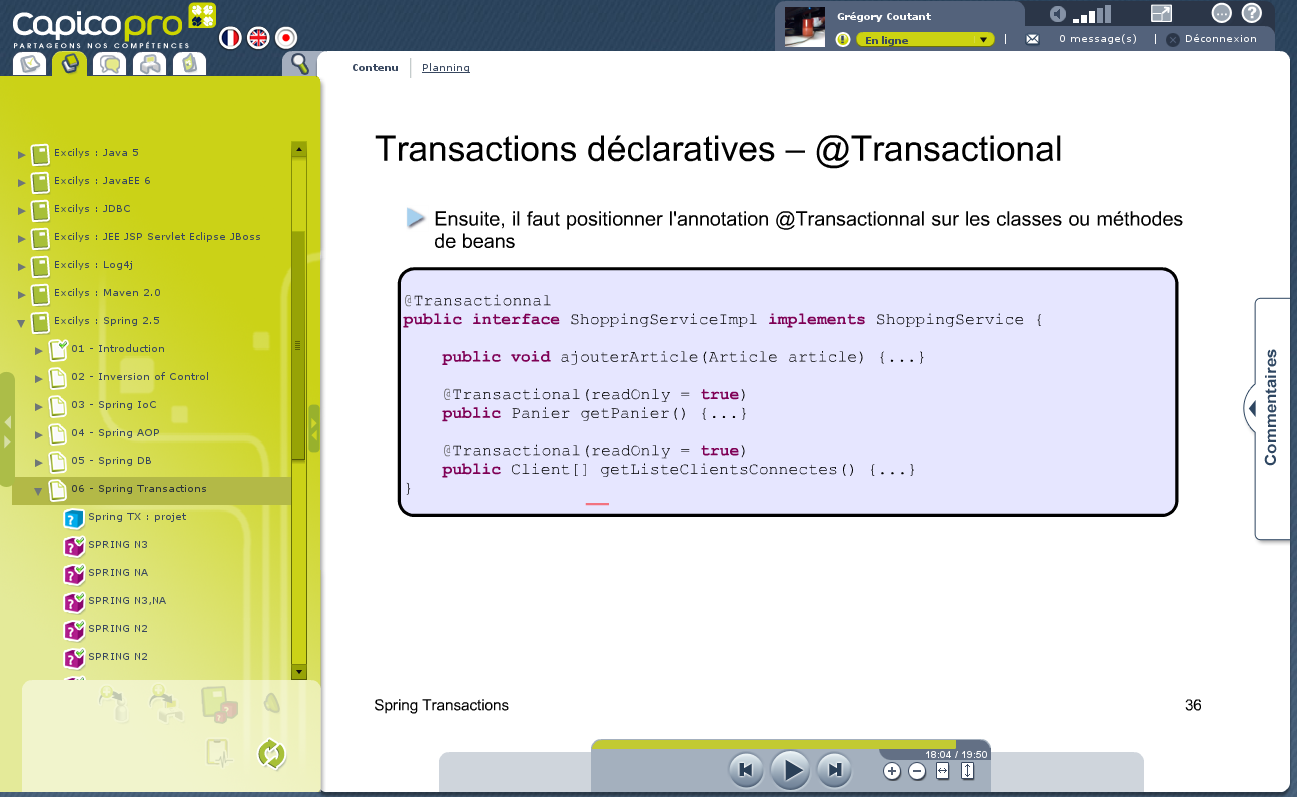
\includegraphics[width=\linewidth]{images/capico.pdf}
	\caption{Éxemple de cours sur Capico}
\end{figure}

Stéphane LANDELLE est responsable de la formation des stagiaires. Il s'assure donc du bon suivi de la formation et la ponctue d'interventions visant à vérifier nos connaissances ou à éclaircir certains points qui pourraient être compliqués. Il permet aussi d'apporter un point de vue plus pratique sur ces technologies, notamment comment elles sont utilisées dans le monde de l'entreprise ou comment elles devraient l'être.

\subsection{Technologies abordées}

Les technologies abordées lors de la formation étant en partie utilisées pendant le reste du stage, je vais maintenant les présenter brièvement pour une meilleure compréhension de la suite du rapport.

\subsubsection{eXtreme Programming (XP)}

XP est une méthode Agile utilisée dans le développement logiciel assez proche d'une autre méthode Agile plus connue : la méthode Scrum \cite{scrum}. Elle découpe le développement d'une application en plusieurs sprints d'une à deux semaines. Le développement est ainsi incrémental garantissant la sortie d'une application fonctionnelle à chaque fin de sprint. Le développement incrémental permet d'avoir un développement plus souple.\\

XP s'appuie notamment sur le pair programming qui consiste à travailler en binôme sur un même ordinateur avec un \emph{pilote} qui contrôle le clavier et la souris et un \emph{copilote} qui a plus de recul et aide le \emph{pilote}. Régulièrement, les rôles s'inversent.\\

Un autre principe de cette méthode est le Test Driven Development (TDD). TDD vise à rendre le développement plus simple et efficace en écrivant d'abord les tests permettant de garantir qu'une fonctionnalité a été développée puis de développer la fonctionnalité. L'idée est de simplement écrire le code qui garantie que les tests passent. Cette méthodologie vise à écrire du code de qualité et fonctionnellement correct, et de faciliter la maintenance de celui-ci. 

\subsubsection{Maven}

Maven \cite{maven} est un outil de gestion et de construction de projets Java. Une de ses forces est notamment de gérer les librairies externes ou bien la sortie d'une nouvelle version. Maven permet d'automatiser la plupart des tâches liées à un projet informatique : récupération des librairies externes, compilation, exécution des tests, génération des livrables, déploiement de l'application sur un serveur, \dots Ce type d'outil est quasiment indispensable pour un projet Java. Maven est la solution la plus utilisé mais d'autres alternatives existe comme Ant ou Gradle. 

\subsubsection{Java}

Java \cite{java} est un langage de programmation orienté objet développé par Sun Microsystems (racheté par Oracle Corporation). Il est vraisemblablement le langage les plus utilisé en entreprise. C'est un langage compilé qui s'exécute sur une machine virtuelle appelée Java Virtual Machine (JVM), ce qui permet aux applications Java d'être portables puisque seule la JVM dépend du système d'exploitation.\\

Un des principe fondamental de Java qui fait de lui un langage très apprécié des entreprise est la garantie de la rétro-compatibilité entre différentes versions de Java. Ainsi une application développée en Java 1.4 peut fonctionner sur une JVM Java 7, profitant ainsi des améliorations apportées à celle-ci.

\subsubsection{JUnit}

JUnit \cite{junit} est un framework permettant d'effectuer facilement des tests unitaires. C'est actuellement le framework le plus utilisé pour les tests dans le monde Java ce qui lui permet d'être très bien intégré dans les environnements de développement tels qu'Eclipse, ou dans des outils comme Maven.

\subsubsection{Java Enterprise Edition (JEE)}

JEE \cite{jee} est une plateforme de développement d'applications d'entreprise décrite par un ensemble de spécifications (28 spécifications pour JEE 6) appelées JSR permettant de normaliser les technologies utilisées telles que :

\begin{description}
	\item[Servlets] objets Java capable de répondre à des requêtes HTTP,
	\item[Java Server Pages (JSP)] langage permettant de générer dynamiquement des pages HTML en s'interfaçant facilement avec du code Java,
	\item[Java Persistence API (JPA)] API inspirée d'Hibernate, permettant de persister dans une base de données relationnelle des objets Java,
	\item[Entreprise JavaBean (EJB)] architecture coté serveur servant à créer des composants distribuées.
\end{description}

\subsubsection{Java DataBase Connectivity (JDBC)}

JDBC \cite{jdbc} est une API permettant la communication avec des bases de données relationnelles. JDBC permet de s'abstraire du langage de requêtes utilisé par la base de données. La traduction des requêtes se fait en temps réel par le pilote spécifique à la base de données utilisée.

\subsubsection{Hibernate}

Hibernate \cite{hibernate} est un framework d'Object Relational Mapping (ORM), c'est à dire un framework permettant de faire la passerelle entre une représentation objet d'un modèle et sa représentation relationnelle. Il permet ainsi de persister de façon simple et intuitive les objets Java dans une base de données relationnelle. Hibernate s'occupe de faire le lien entre les classes et attributs Java et les tables d'une base de données. Depuis sa version 4, Hibernate est une des implémentation de JPA.

\subsubsection{Spring}

Le framework Spring \cite{spring} est une alternative et un concurrent à la plateforme JEE. L'idée est de proposer au développeur un ensemble de fonctionnalités à la manière de JEE mais sous la forme de dépendances modulaires. Ainsi, une application Spring peut fonctionner sur une simple JVM ou sur un serveur léger tel que Tomcat ou Jetty. Au contraire d'une application JEE qui se déploie uniquement dans un conteneur lourd, ou serveur d'application, tel que Glassfish ou JBoss implémentant toutes les JSR de la spécification JEE. Les applications JEE sont extrêmement dépendantes du conteneur ce qui restreint la portabilité de l'application, à la différence d'une application Spring.\\

Le c\oe{}ur de Spring est une implémentation du design pattern Inversion of Control (IoC) : l'instanciation des classes n'est plus à la charge du développeur mais du framework. Ceci permet ainsi de l'injection de dépendance, c'est à dire, d'automatiquement injecter à l'exécution les dépendances d'un objets lors de son instanciation. On peut donc modifier le comportement de l'application à l'exécution. Tous les modules de Spring reposent sur cette fonctionnalité. La déclaration des instances gérées par Spring se fait via un fichier XML ou via des annotations directement dans le code. On peut donc voir Spring comme une fabrique d'objets (design pattern Factory).\\

De nombreux modules font de Spring une énorme boite à outils : intégration avec un ORM (Hibernate, JPA, \dots), programmation orientée aspect (AOP), implémentation du design pattern MVC pour faciliter la création d'application web, intégration dans les frameworks de tests unitaires (JUnit), \dots

\subsection{Formation continue}

Après la phase de formation du stage terminée, j'ai ,parallèlement au travail demandé, continué et approfondi plusieurs sujets pour ma curiosité personnelle mais aussi parce que c'est un des devoirs d'un consultant du \excilysGroup{}.\\

En premier lieu, j'ai approfondi mes connaissances en Java pure pour notamment pouvoir passer l'examen d'Oracle Certified Java SE 6 Programmer (OCJP). Cet examen permet d'être certifié par Oracle comme \flqq{}maîtrisant le langage Java\frqq{} si le score obtenu est supérieur à 61 \%. Cette certification est nécessaire pour être embauché dans le \excilysGroup{}. J'ai obtenu la note de 91 \%.\\

En second lieu, je me suis aussi intéressé à des technologies émergentes comme Scala, Play! 2 ou bien Gradle.

\section{Mini-projet d'e-banking}

À la suite de notre formation, nous avons mis en pratique nos connaissances dans un mini-projet de réalisation d'une application web d'e-banking.

\subsection{Cahier des charges}

L'application à réaliser est une application web de gestion des comptes. Les fonctionnalités sont les suivantes :

\begin{itemize}
	\item S'identifier,
	\item Consulter la liste de ses comptes,
	\item Consulter le détail des opérations pour un compte et un mois donné,
	\item Consulter le détail des opérations cartes pour un compte et un mois donné,
	\item Effectuer un virement entre ses comptes,
	\item Consulter l'historique de ses virements,
	\item Exporter au format Excel le relevé des opérations pour un mois donné.
	\item Exposer ces fonctionnalités sous la forme de web services.
\end{itemize}

\subsection{Gestion du projet}

Étant cinq stagiaires à être arrivés le même jour et un autre la semaine suivante, nous avons formé une équipe de six personnes pour réaliser ce projet. Il nous avait été laissé la possibilité de former deux groupes projet de trois personnes, mais nous avons préférer former une seule équipe et ainsi avoir la possibilité d'approfondir de façon plus importante le projet.\\

La méthode que nous avons utilisé pour gérer ce projet a été un mélange entre la méthode Scrum et l'XP, soit deux méthodes Agiles. L'utilisation des méthodes Agiles repose en grande partie sur le constat qu'un produit logiciel voit la plupart du temps ses demandes en fonctionnalités évoluer au fur et à mesure, et que cela est très difficile à prendre en compte avec un  système non itératif, comme pas exemple le cycle en V. Ici, le but est d'effectuer de courtes itérations d'une à deux semaines au bout desquelles un produit utilisable est livré. Dans notre cas, du fait de la durée du projet, nous avons fait des itérations (ou sprints) d'une semaine.\\

La première itération, appelé Sprint 0 a consisté en la mise en place de l'environnement de développement, de l'environnement d'intégration ainsi que des conventions à utiliser. C'est au cours de cette semaine que nous avons aussi choisi le socle de technologies que nous utiliserions. Nous avons aussi réfléchi à l'architecture générale de l'application. Tous ces choix sont expliqué dans la suite du rapport. À la fin de ce premier Sprint, nous avons fait une réunion avec Stéphane LANDELLE, le directeur technique d'\ebi{}, pour valider nos choix.\\

Les autres itérations ce sont ensuite déroulées de la façon suivante :
\begin{enumerate}
	\item Réunion avec le \flqq{}product owner\frqq{} (client dans le vocabulaire Scrum), c'est à dire Stéphane LANDELLE, pour sélectionner les fonctionnalités à développer dans cette itération,
	
	\item Développement des fonctionnalités, principalement en pair programming pour mutualiser les connaissances,
	
	\item Réunion technique avec Stéphane LANDELLE en tant que référent technique pour auditer notre code,
	
	\item Remaniement (refactoring) du code suite aux remarques.
	
	\item Réunion avec le \flqq{}product owner\frqq{} pour présenter les fonctionnalités implémentées.\\
\end{enumerate}

De plus, chaque jour nous réalisions un \flqq{}daily Scrum\frqq{} à heure fixe : c'est une courte réunion dans laquelle tout les intervenants sont debout, pour pousser à la concision, et répondent à trois questions :
\begin{enumerate}
	\item Qu'est-ce que j'ai fait hier ?
	
	\item Qu'est-ce que je compte faire aujourd'hui ?
	
	\item Quelles sont les difficultés que je rencontre ?\\
\end{enumerate}

Cette méthode permet d'avoir un résultat chaque semaine à montrer au client. Le client peut donc voir l'évolution du projet en temps réel, tester les parties déjà développées ce qui permet d'avoir un retour rapide. De plus, le client est beaucoup plus investi dans le projet et peut facilement ajuster ou modifier le cahier des charges.\\

Pour le développeur, les itérations permettent de ne pas avoir un travail trop répétitif puisque dans chaque itération, on retrouve toutes les phases du cycle en V classique. Il n'y a donc plus de grandes phases de développement, de tests, de recette, \dots{}

\subsection{Choix techniques}

Le choix des technologies à utiliser était en grande partie libre, même s'il était soumis à l'approbation de Stéphane. Voici les technologies que nous avons choisi :

\subsubsection{Gestionnaire de version}

Il permet de travailler sur un projet de manière collaborative et simultanée. Il existe principalement deux gestionnaires de version : Git et Subversion, dont la philosophie diffère.\\

Subversion est le plus répandu actuellement car plus ancien. C'est un système de versionnement centralisé, i.e. qu'il n'existe qu'un seul dépôt des versions, robuste qui à fait ses preuves. Le développement est fortement linéaire, car la création d'une branche demande la copie complète du code.

Git est lui plus récent (2005). Il a été créé par Linus Torvalds pour gérer le développement du noyaux Linux. C'est un système de versionnement décentralisé, chaque utilisateur dispose d'un dépôt local, très puissant. Il tire profit au maximum des branches pour avoir des fonctionnalités se développant en parallèle sans rentrer en conflit. Une fois une fonctionnalité développée sa branche est fusionnée à la branche principale généralement appelée master.\\

Nous avons choisi d'utiliser Git, car même si ce n'est pas actuellement le système le plus utilisé, la puissance et la flexibilité qu'il apporte en feront surement le leader dans un futur proche. De plus l'utilisation de cette outil nous a permis de mettre en place un processus d'intégration continue très intéressant qui sera détaillé ci-après. Malgré son coté décentralisé nous avions besoin d'un dépôt distant permettant de centraliser le travail et d'accéder au code de n'importe où. Nous avons ainsi choisi d'héberger notre projet sur GitHub, plateforme d'hébergement de projet open-source utilisant Git. 

\subsubsection{Construction du projet}

Plusieurs systèmes permettent de construire des projets Ant, Maven, Gradle, \dots{} Ant est le plus ancien. C'est globalement un outil qui permet d'écrire des scripts pour construire des applications. Il est très apprécié car il est très flexible.\\

Maven est plus récent, s'appuie sur des script de build en XML, et se base sur le principe de \flqq{}convention over configuration\frqq{}, c'est à dire qu'il encourage le développeur à respecter certaines conventions pour faciliter la construction du projet comme par exemple l'arborescence du projet, i.e. emplacement des sources, des sources de test \dots{}. Il inclut aussi un système de gestion de dépendance qui va directement chercher les librairies externes dans des dépôts Maven accessibles publiquement.\\

Gradle quant à lui est le plus récent. Il reprend beaucoup des principes de Maven, notamment la gestion des dépendances et le principe de \flqq{}convention over configuration\frqq{}, mais permet aussi une plus grande flexibilité se rapprochant ainsi plus de Ant, grâce à des script écrit en Groovy.\\

Nous avons choisi Maven car c'est actuellement le plus utilisé en entreprise et qu'il est pour des projets relativement classique le plus abouti.

\subsubsection{Système de Gestion de Base de Données (SGBD)}

Afin de persister nos données nous avons besoin d'un SGBD. Il existe de nombreuses possibilités et l'application à réaliser n'a pas besoin de fonctionnalités avancées hormis une gestion des transactions pour garantir la cohérence de nos tables.\\

Les deux principaux SGBD open source sont MySQL et PostgreSQL. Ces deux solutions sont assez proches. Nous avons choisi PostgreSQL pour son plus grand respect de la norme SQL.

\subsubsection{ORM}

Le choix de d'Hibernate comme ORM nous a été imposé. En effet il est actuellement le standard de facto et sa maitrise est un impératif de notre métier. Nous avons par contre choisi d'utiliser la version 4, qui est une implémentation de la spécification JPA. Il est a noter que l'implémentation de référence de cette spécification est TopLink, mais qu'elle est beaucoup moins utilisée. 

\subsubsection{Conteneur d'application}

Les conteneurs d'applications sont des boites à outils fournissant des services pour résoudre des problématiques que toute application rencontre. Dans le monde Java, il en existe principalement deux : JEE et Spring.\\

A nouveau le choix de Spring nous a été imposé. Car même si il n'est pas porté par un standard Spring est le conteneur le plus répandu dans le monde de l'entreprise. Spring est un conteneur léger qui ne nécessite pas un serveur d'application mais un simple conteneur de Servlet contrairement au conteneur JEE. Ceci permet d'éviter, au moins pour le développement de l'application, la complexité, la lenteur et la lourdeur de serveur comme JBoss, Weblogic ou Websphere et de simplement déployer son application dans un Tomcat ou un Jetty qui sont beaucoup plus rapide.\\

De plus, nous avons aussi utiliser Spring pour l'intégration d'Hibernate (Spring-DB), la gestion des transactions (Spring-TX), le framework MVC (Spring-MVC), la sécurité (Spring-Security) et la mise en place de traitement batch (Spring-Batch). 

\subsubsection{Serveur}

Puisque nous utilisons Spring, nous pouvons utiliser un simple conteneur de Servlet. Il en existe principalement deux Jetty et Apache Tomcat. Nous avons préféré Tomcat car encore une fois, il est le plus répandu et que sa robustesse n'est plus a démontrer. Il sert entre autre de conteneur de Servlet dans le serveur JBoss et sert par exemple en production chez Atos Worldline. 

\subsubsection{Frameworks de tests}

Les tests sont une composante importante d'un projet informatique. Il existe différents types de tests qui répondent à différentes problématique.

Tout d'abord les tests unitaires qui vont permettre de s'assurer du bon fonctionnement et de la non régression d'un composant logiciel. Dans ce but nous avons utilisé JUnit, qui est le standard de facto dans le monde Java. D'autre alternative existe comme TestNG qui d'un point de vue strictement technique est plus performant. Mais la prédominance de JUnit dans le monde professionnel nous a fait préférer cette solution.\\

Pour pouvoir isoler les composants logiciel lors des tests unitaires nous avons aussi utilisé un framework de mock. Mocker un objet consiste à remplacer un objet par un faux dont on fixe le comportement. Si par exemple une classe A utilise une autre classe B pour son fonctionnement. Lorqu'on veut tester uniquement la classe A, il faut mocker la classe B et injecter le mock dans la classe A. Ainsi les bugs dans la classe B n'interfèrent pas avec les tests de la classe A. Pour cela nous avons utilisé Mockito qui nous a été recommandé par Stéphane. Les autres possibilités sont EasyMock ou PowerMock. L'avantage de Mockito par rapport à Easymock est que nous ne sommes pas obligé de spécifier de façon exhaustive le comportement du mock.\\

Ensuite il existe les tests d'intégration qui vont permettre de tester fonctionnellement l'application et ainsi s'assurer du bon comportement général. Notre choix s'est porté sur Selenium. Ce framework permet de jouer des actions utilisateurs comme des clics sur un bouton, le remplissage de formulaires, et de spécifier un certain nombre de contrôles pour vérifier le bon comportement.

Enfin nous avons aussi réalisé des tests de monté en charge grâce à Gatling. C'est tests visent à s'assurer du bon fonctionnement de l'application lorsque celle-ci est utilisée en simultané par une population d'utilisateur.

\subsubsection{Serveur d'intégration}

Un serveur d'intégration est un serveur qui périodiquement récupère le code source d'un projet depuis un gestionnaire de version, le construit, exécute les tests unitaires et les tests d'intégrations et génère un rapport avec le résultat de la construction du projet et de l'exécution des tests. Ce serveur permet d'avoir un système d'intégration continue : lorsqu'un développeur modifie le code source et envoie ses modifications au gestionnaire de version, le serveur d'intégration va permettre de vérifier qu'il n'y ait pas de régression et garantir le bon fonctionnement de l'application.\\

Nous avons choisi d'utiliser Jenkins (anciennement Hudson) car c'est le serveur d'intégration open source le plus utilisé dans le monde Java. Il est entre autre la pierre angulaire du PaaS (Platform as a Service) de CloudBees DEV@Cloud.

\subsubsection{Framework de web services}

Les web services sont des services distribués utilisant HTTP comme protocole de transport. Ces web services permettent à une application tierce d'interagir avec notre application. Il existe principalement deux types de web services : SOAP (Simple Object Access Protocol) et REST (REpresentational State Transfer).\\

SOAP est un standard qui s'appuie principalement sur XML ce qui fait de lui un protocole très verbeux et est généralement utilisé dans un même réseau, c'est à dire entre des applications d'un même système d'information par exemple.\\

REST n'est pas à proprement parlé un protocole mais simplement un type d'architecture : puisqu'on utilise HTTP pour le transport, utilisons toutes les possibilités de ce protocole. Il est généralement utilisé en combinaison avec JSON (JavaScript Object Notation) permettant de représenter les objets sous la forme de chaîne de caractères.\\

Pour la mise en place des web services nous avons choisi Apache CXF puisqu'il permet de faire des web services SOAP et REST en implémentant les respectivement les spécification JaxWS et JaxRS et s'intègre complètement avec Spring.

\subsubsection{Autres technologies}

Nous avons utilisées d'autres technologies sur lesquelles je ne m'étendrai pas sur le choix :

\begin{description}
	\item[JSTL] Fourni un ensemble de tags pour faciliter l'écriture de pages JSP avec notamment des boucles et des blocs conditionnelles tout en restant complètement du code XML,
	
	\item[Liquibase] Permet de versionner la base de données en écrivant des scripts XML agnostique de la BDD s'exécutant lors du déploiement de l'application garantissant ainsi la cohérence entre l'application et le schéma de la base de données,
	
	\item[Twitter Bootstrap] Feuille de style CSS pour créer des pages HTML avec un design propre de façon simple et rapide.
	
	\item[EHcache] Cache Java distribué. Le cache permet par exemple de soulager la base de données en gardant en mémoire le résultat d'un certain nombre de requête évitant ainsi d'interroger la base à chaque fois.\\
	
	
\end{description}

Ces technologies ont été choisies principalement car elles sont très répandues dans le monde de l'entreprise. Ce mini-projet nous a donc permis de nous faire la main sur les technologies que nous sommes le plus à même de rencontrer en clientèle.

\subsection{Architecture de l'environnement de développement}

Build incassable
Intégration des tests.

\subsection{Architecture du projet}

Au cours de la première itération nous avons choisi l'architecture à mettre en place pour réaliser notre application. Nous avons choisi d'utiliser une architecture 3-tiers classique. La couche de présentation est implémentée avec le design pattern MVC. Une architecture 3-tiers découpe l'application en 3 couches :

\begin{description}
	\item[Persistance] Contient les DAO (Data Acces Object), c'est à dire les classes interagissant directement avec l'ORM pour persister les objets dans la base de données ou pour les récupérer,
	
	\item[Application] Contient la logique métier de l'application,
	
	\item[Présentation] Permet la présentation des données à l'utilisateur. La couche de présentation est souvent implémentée avec le design pattern MVC qui permet de facilement séparer les données à afficher, la façon de les afficher et les interactions entre le système et l'utilisateur.
\end{description}

\begin{figure}[H]
	\centering
	\includegraphics[width=0.7\linewidth]{images/architecture.pdf}
	\caption{Architecture de l'application}
\end{figure}

Une telle architecture repose sur un principe très simple : une couche utilise uniquement la couche inférieure, ce qui permet de pouvoir séparer les problématiques telles que l'accès aux données, la logique métier, \dots{} On peut aussi remarquer l'ajout des web services qui, à la manière de la couche de présentation, se greffe au-dessus de la couche application.\\

D'un point de vue Maven, nous avons découpé le projet en sous modules Maven pour pouvoir facilement construire des parties du projets sans avoir à tout reconstruire. Les sous modules sont les suivants :

\begin{description}
	\item[backend] Contient les couches de persistance et application,
	\item[frontend] Contient la couche de présentation,
	\item[web services] Contient les web services.\\
\end{description}

Le backend est un JAR (Java ARchive) spécifié en tant que dépendance des deux autres sous modules. Le frontend est un WAR (Web ARchive) tout comme les web services. L'avantage de ce découpage est qu'il nous permet de déployer sur un serveur uniquement le frontend, c'est à dire l'application web à proprement parlé, ou uniquement les web services ou les deux.

\subsection{Itérations}

Je vais maintenant passé en revue les différentes itérations pour expliquer dans quel ordre nous avons développé les fonctionnalités.

\subsubsection{Itération 1}

Pour la première itération, nous avons mis en place la fonctionnalité qui nous semblait absolument nécessaire pour pouvoir développer le reste à savoir la connexion en tant qu'utilisateur. Pour cela nous avons donc commencé à mettre en place la base de données avec la liste des utilisateurs et les rôles, c'est à dire, les simple utilisateurs ou les administrateurs. La connexion est gérée via un module Spring appelé Spring Security.

\subsubsection{Itération 2}

Nous avons ensuite développé la consultation de la liste des comptes ainsi que du résumé de chaque compte par mois. Pour ce faire, nous avons implémenté un système de pagination très important dans beaucoup d'application web. En effet, un système de pagination permet de ne pas surcharger les échanges réseaux ainsi que le volume de données à charger depuis la base de données. Dans notre cas, la pagination sert à n'afficher qu'un nombre défini d'opérations pour un compte et un mois donné.

\subsubsection{Itération 3}

Lors de cette troisième itération, nous avons mis en place les virements. Nous en avons profité pour revoir le fonctionnement de l'application pour s'assurer que celle-ci ne génère que des pages \flqq{}bookmarkable\frqq{} avec des URL simples. Des pages bookmarkable, impliquent que si un utilisateur enregistre l'URL de la page, il doit pouvoir y retourner sans problèmes. Cela veut dire que les pages affichées ne dépendent pas des pages consultées auparavant. Suivre ce principe, permet de rendre l'application plus intuitive et facile d'accès.

\subsubsection{Itération 4}

Durant cette dernière itération, nous avons mis en place les web services SOAP et REST.

\subsection{Produit final}

\begin{figure}[H]
	\centering
	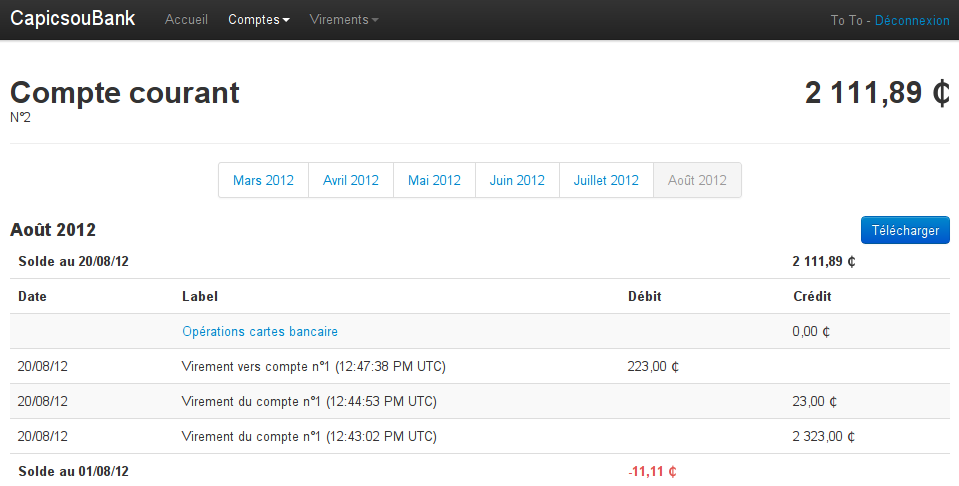
\includegraphics[width=\linewidth]{images/capicsoubank.pdf}
	\caption{Résumé du compte pour le mois d'août}
\end{figure}

L'application est disponible à l'adresse : \url{http://capicsoubank.j.layershift.co.uk}. Pour se connecter, on peut utiliser le compte avec le nom d'utilisateur \verb+toto+ et le mot de passe \verb+toto+.\\

Cette application nous aura permis de terminer notre formation, en nous faisant la main sur les technologies les plus utilisées dans le monde de l'entreprise. Cette application nous a aussi forcé à faire attention à la façon d'implémenter certains aspects d'une application web, notamment à faire attention aux nombres de requêtes par page.\\

Bien que nous n'avions aucun impératif de performance, nous nous sommes restreints au strict nécessaire en terme d'accès base de données pour garantir un bon fonctionnement, même avec une charge sur le serveur.\\

Enfin, l'utilisation des méthodes Agiles nous a permis de développer rapidement sans avoir le réflexe de tout prévoir avant de véritablement implémenter les fonctionnalités. Avec les méthodes Agiles et toutes les méthodes fonctionnant en itération, il ne faut pas développer plus que nécessaire pour la fonctionnalité en cours. L'avantage est de ne pas avoir de code qui sera peut être utilisé plus tard et qui, en réalité, deviendra très certainement du code mort.


\section{Gatling}

Après le projet d'e-banking, j'ai rejoint, avec deux autres stagiaires, Stéphane LANDELLE sur son projet open-source appelé Gatling \cite{gatling} pour le restant de mon stage.

\begin{figure}[H]
 \centering
 
\includegraphics[width=0.3\linewidth]{images/logo_gatling.pdf}
\end{figure}


\subsection{Présentation du projet}

\subsubsection*{Qu'est-ce que Gatling ?}

Gatling \cite{gatling} est un outil permettant de réaliser des tests de charges, par exemple sur des applications web. Ce projet est dans sa grande majorité open-source. Il a été créé par Stéphane LANDELLE, directeur technique d'\ebi{}, en Janvier 2012 et est activement soutenu par le \excilysGroup{}.

Un outil de tests de charge permet de simuler le comportement d'un nombre arbitraire d'utilisateurs pour pouvoir tester le comportement d'une application face à une utilisation simultanée, proche des conditions d'utilisation réelles. Ce type d'outil a pour but de détecter les problèmes de performance d'une application avant sa mise en production.

\subsubsection*{Pourquoi avoir créé Gatling ?}

Avant la création de Gatling il existait déjà de nombreux injecteurs de charge comme :

\begin{itemize}
	\item JMeter
	\item LoadUI
	\item LoadRunner
	\item The Grinder
	\item etc\ldots \\
\end{itemize}

Alors pourquoi créer un nouvel outil ? Car aucun de ceux-ci n'avait satisfait Stéphane LANDELLE lors de ses différentes mission. Il a donc pensé qu'il y avait une place pour un nouvel injecteur qui répondrait à ses attentes.\\

Les principaux inconvénients des solutions existantes sont :

\begin{itemize}
	\item Le cout de la licence pour les solutions payantes : 10000\$ dans le cas de LoadUI.
	\item Le manque d'activité et de maintenance du projet par exemple pour The Grinder. 
	\item Les problèmes de performance de certains outils qui demande donc une ou plusieurs machines très puissantes pour être efficace. 
	\item L'écriture des scénarios de tests en XML, ce qui les rend peu lisible et maintenable, ce qui est le cas de JMeter.\\
\end{itemize}

Gatling a donc été mis au point afin d'offrir une alternative, venant corriger ces problèmes.

\subsubsection*{Qu'est ce qui différencie Gatling de ces concurrents ?}

Le modèle des \textit{acteurs} sur lequel repose Gatling ainsi que son utilisation des communications asynchrones font de Gatling un outil peu gourmand en ressources.
JMeter, son principal concurrent dans l'écosystème Java, exigera une ou des machines très puissantes pour injecter une charge que Gatling peut effectuer sur une machine aux performances modérées.\\

Une autre différence importante entre Gatling et certains de ses concurrents est le format des scénarios de tests (ou \textit{simulations}).\\
Alors que de nombreux outils utilisent un fichier au format XML afin de décrire leur simulations, ce qui les rend plus difficilement lisible et manipulable sans passer par l'UI de l'outil et également plus difficilement maintenable, les simulations de Gatling sont écrits  à l'aide d'un DSL (Domain-Specific programming Language) basé sur Scala, simples à modifier, à mettre à jour et à intégrer au reste du projet (dans le cadre d'un système de contrôle de version par exemple).

\begin{figure}
 \centering
 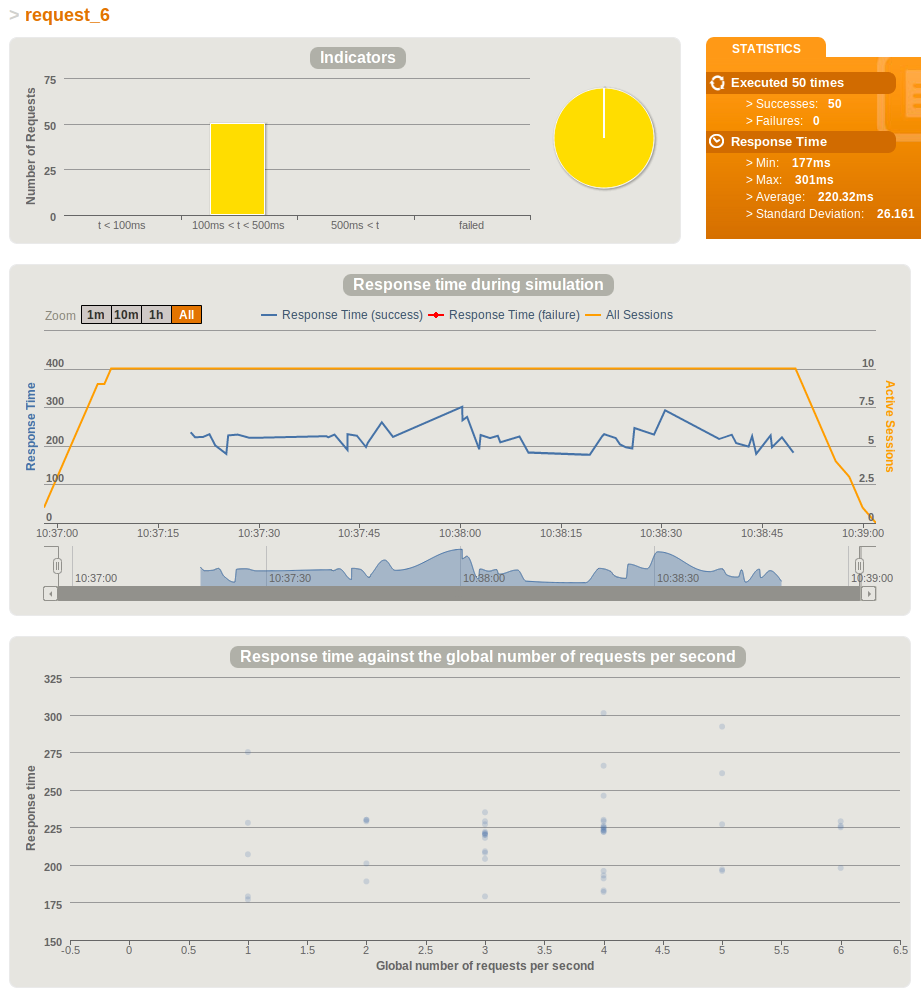
\includegraphics[width=\linewidth]{images/req_details_basic_usage.pdf}
 \caption{Exemple de rapport pour une requête}
\end{figure}

\subsection{Technologies utilisées}

Le projet est lui-même écrit en Scala, un langage de programmation multi-paradigme. Il utilise Akka une librairie Scala/Java permettant de créer facilement des applications concurrentes. Gatling repose pour les I/O sur la librairie Async IO basé sur Netty.

\subsubsection{Scala}

Gatling est écrit en Scala \cite{scala}, un langage qui mélange les paradigmes de programmation orienté objet et de programmation fonctionnelle. Ce langage a été créé en 2003 par Martin ORDERSKY, qui a aussi travaillé sur \verb+javac+, le compilateur Java. Ce langage qui a presque 10 ans connait ces dernières années une augmentation rapide de sa popularité grâce à son utilisation chez Twitter et à la création de framework comme Akka ou Play \cite{play} qui permettent de créer des applications web uniquement en Scala.\\

Comme en Java, le code Scala est compilé en bytecode et est exécuté sur une JVM. Scala et Java sont interopérable puisqu'il est possible d'utiliser des API Java en Scala et inversement. D'ailleurs, de nombreuses API du SDK Java n'ont pas d'équivalent en Scala, il suffit d'accéder directement à l'API Java.\\

Scala est un langage fortement typé au même titre que Java, cependant le type des variables peut être inféré à la compilation. De plus il tire beaucoup plus partie de la généricité. C'est à dire le fait de paramétrer une classe ou une fonction par un type. L'objectif étant d'avoir un maximum d'erreur de type découvert par le compilateur et non à l'exécution.\\

Un des avantages de Scala est l'écriture d'un code beaucoup plus concis qu'en Java, au prix d'une compilation plus lente. Le code Scala est plus concis car il permet d'éviter d'écrire toute la partie du code qui n'est pas réellement utile et qui devient donc facultative.\\

Ce langage permet d'écrire un code vraiment réduit à son essence, ce qui permet de le rendre plus maintenable. Sa compréhension peut être cependant plus complexe. De plus, la façon de développer et penser son code est différente de celle de Java puisqu'on est aussi dans un paradigme de programmation fonctionnelle.\\

Il a donc nécessité un temps d'adaptation et d'apprentissage \cite{proginscala} avant de pouvoir comprendre le fonctionnement interne de Gatling et de pouvoir développer de nouvelles fonctionnalités.

\subsubsection{Akka}

Akka \cite{akka} est un framework écrit en Scala, disposant aussi d'une API Java, pour faciliter la réalisation d'applications fortement concurrentes en s'appuyant sur le système des Acteurs. Le framework Akka permet de s'abstraire de la notion de threads et d'exploiter au maximum les processeurs multi-cœurs. Dans le cas de Gatling, l'objectif est de pouvoir gérer un grand nombre d'utilisateurs en parallèle.\\

Akka utilise, pour s'abstraire des threads et régler les problèmes de synchronisation liés à la concurrence, le système des acteurs. Les acteurs sont des objets encapsulant un état et un comportement. Ils communiquent entre eux exclusivement à l'aide de messages placé dans une boite au lettre propre à chaque acteur. L'exécution d'un acteur est démarré par la réception d'un message. Ceci permet de réaliser la plupart des traitement de manière asynchrone et de minimiser ainsi le blocage des threads. En effet un acteur n'est pas lié à un thread, il est exécuté sur un thread quelconque lorsque cela est nécessaire. En interne, Akka utilise un pool de threads pour exécuter les acteurs. Ceci permet d'avoir potentiellement un très grand nombre d'acteurs qui s'exécutent (plus de 1000) sur un pool de threads restreints (30 threads).

\subsubsection{Netty \& Async HTTP Handler}

Async HTTP Handler est un client HTTP reposant sur le moteur Netty qui permet de gérer l'envoi de requêtes (et le traitement des réponses) HTTP de manière asynchrone, complétant ainsi le caractère asynchrone d'Akka, ce qui permet à Gatling de disposer d'un moteur intégralement asynchrone. 

\subsection{Architecture de Gatling}

\begin{center}
	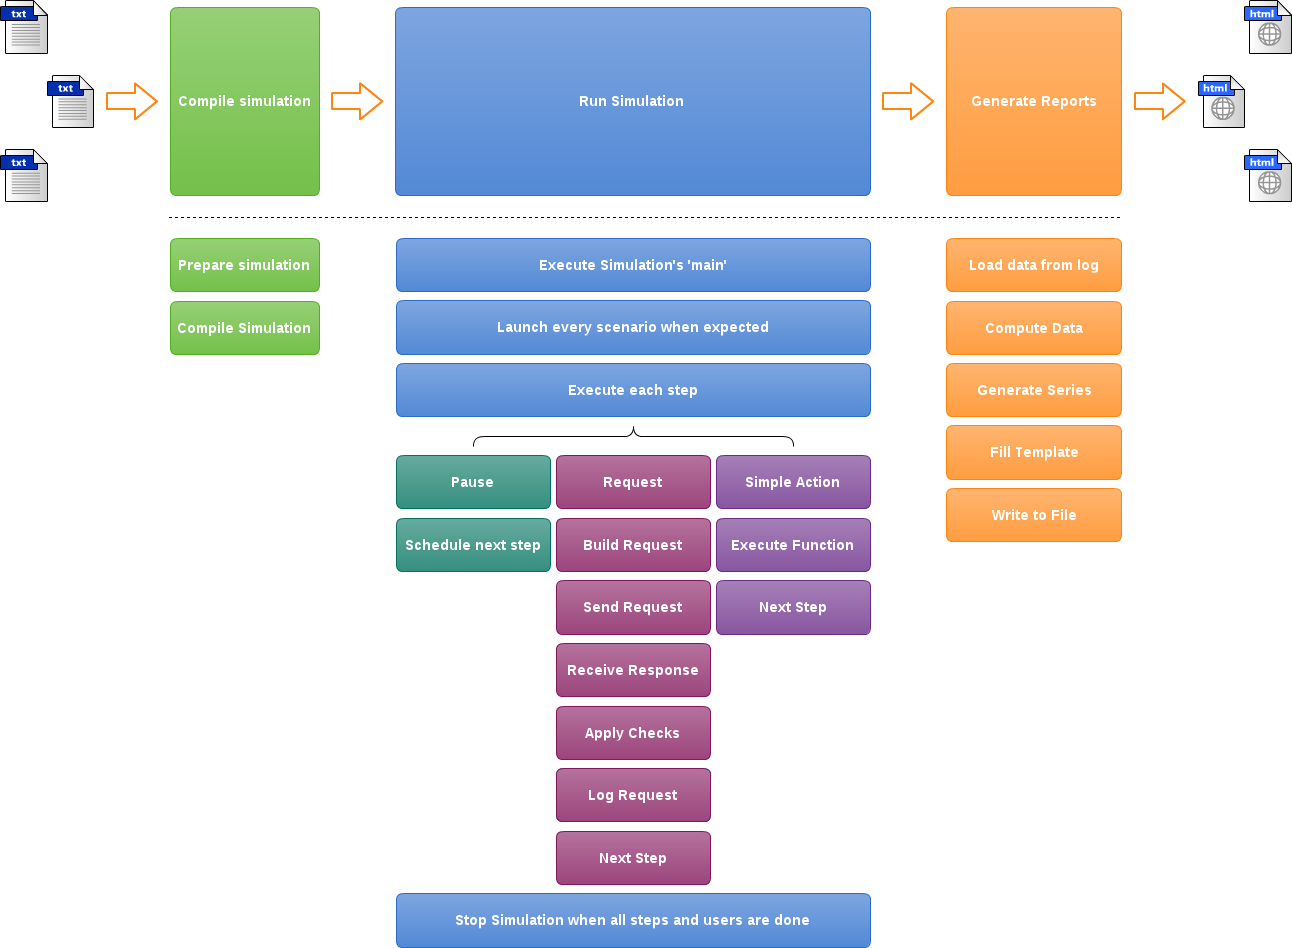
\includegraphics[scale=0.3]{images/gatling-process.pdf}
\end{center}

\subsection{Récupération des métriques serveurs}

Actuellement, les mesures prises par Gatling ne concernent que ce qu'un utilisateur de l'application observerait : le temps que met une page web à répondre ou tout simplement si celle répond ou non.\\

La première fonctionnalité que Stéphane LANDELLE souhaitait que nous étudions été le monitoring de l'application testée, c\^oté serveur.\\

Ce choix était motivé par deux raisons :

\begin{itemize}
	\item Bien qu'étant open source, Gatling reste en concurrence avec d'autres solutions, et plusieurs d'entre elles proposent du monitoring c\^oté serveur ou comptent en intégrer dans un futur proche. Intégrer du monitoring c\^oté serveur  dans Gatling permettrait donc à celui-ci de ne pas prendre de retard sur la concurrence.
	\item Monitorer l'application testée permettrait d'obtenir de précieuses informations sur le comportement de l'application durant le test que ça soit en terme d'utilisation CPU, de mémoire, d'activité des bases de données\ldots En recoupant ces informations avec celles déjà existantes, cela permettrait d'obtenir des rapports encore plus pertinents.\\
\end{itemize}

Pour pouvoir mettre en place cette fonctionnalité, nous avons donc effectué un état de l'art des technologies à utiliser, puis nous les avons testé pour vérifié leur impact sur les performances du serveur instrumenté (cf. annexe~\ref{ann:benchmark}).\\

\subsubsection{Java Management eXtensions}

La première technologie que nous avons trouvé est Java Management eXtensions (JMX) \cite{jmx}. JMX est une API Java qui permet de gérer à distance des applications s'exécutant sur une JVM. Elle permet de récupérer des informations exposées par JMX telles que l'utilisation du CPU par la JVM, mais elle permet aussi d'appeler des méthodes distantes pour par exemple redémarrer des composants.\\

En interne, JMX repose sur RMI (Remote Method Invocation), une API Java qui permet d'appeler des méthodes sur des objets distants. L'utilisation de JMX est extrêmement simple, puisqu'il suffit de créer une interface dont le nom se termine par \verb+MBean+ ainsi qu'une classe implémentant cette interface. Elle sera alors automatiquement exposée par JMX et accessible de l'extérieur.\\

Pour pouvoir facilement accéder aux objets exposés (appelés MBean), nous avons utilisé JVisualVM, un programme fournit avec le JDK (Java Development Kit) d'Oracle. Ce programme permet de monitorer des JVM locales ou distantes en accédant notamment aux MBean.

\begin{figure}[H]
 \centering
 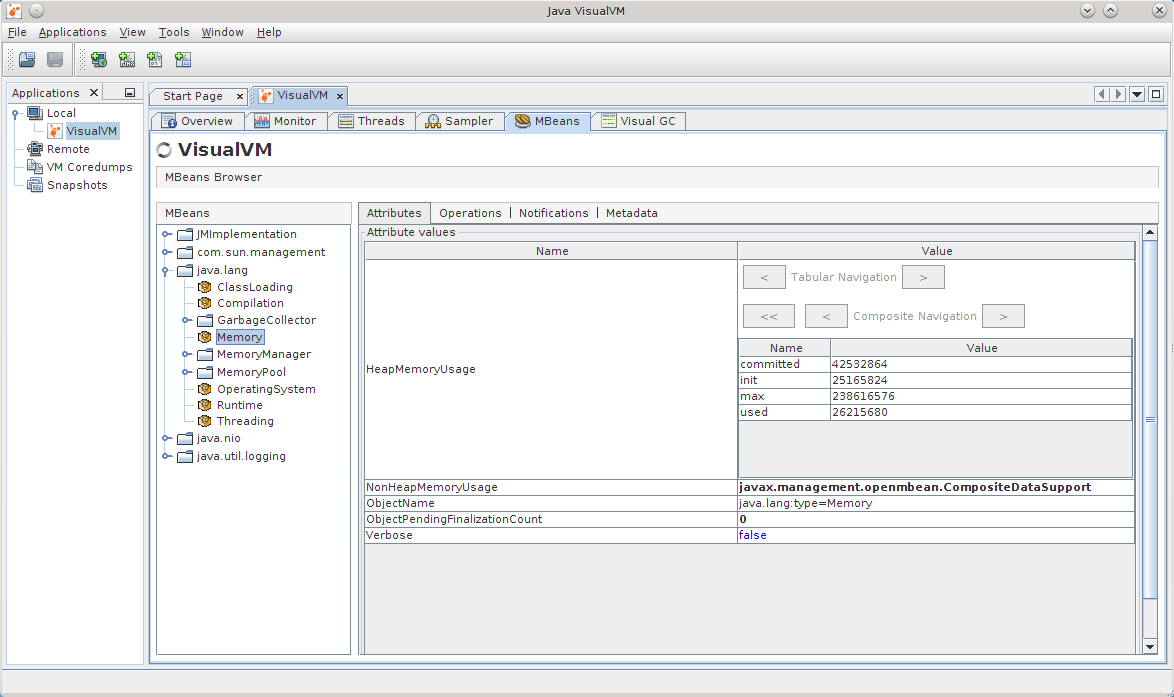
\includegraphics[width=\linewidth]{images/jvisualvm.pdf}
 \caption{Utilisation de JVisualVM pour accéder aux MBean}
\end{figure}


L'utilisation de JMX est donc très simple, de plus, plusieurs métriques sont déjà exposées par la JVM, telle que l'utilisation du CPU, l'utilisation de la Heap (mémore interne de la JVM), la durée totale de collection par le Garbage Collector (GC), \dots{}\\

Cependant, un des inconvénients de l'utilisation de JMX est l'utilisation sous-jacente de RMI qui déclenche régulièrement le GC. L'exécution de celui-ci étant coûteuse en performance, son utilisation peut avoir un impact sur le serveur testé et ainsi fausser les résultats du test de charge.

\subsubsection{Agent Java}

La deuxième technologie est l'utilisation d'un agent java. Un agent java est un code Java qui est exécuté au démarrage de la JVM avant la méthode \verb+main+. Un agent permet notamment de manipuler le bytecode d'une classe au chargement de celle-ci. On peut aussi utiliser un agent pour exécuter du code en parallèle de l'application et donc par exemple, écrire dans un fichier les métriques que l'on veut récupérer.\\

Un des inconvénients des agents est qu'il faut modifier la ligne de commande qui démarre le serveur pour pouvoir ajouter notre agent. Son utilisation est donc assez complexe puisqu'il nécessite une intervention de la personne qui souhaite utiliser Gatling.\\

Cependant, Sun a créé une API permettant d'attacher un agent à une JVM déjà en cours d'exécution. Il est donc possible d'attacher notre code à une JVM de façon assez simple. Cette API possède une limitation puisqu'on ne peut attacher un agent uniquement à une JVM locale et non distante. Son utilisation nécessite donc toujours une intervention de l'utilisateur de Gatling, mais l'intervention est plus simple puisqu'il ne s'agit que d'exécuter un programme qui va découvrir les JVM et attacher l'agent.\\

Un agent permet donc d'exécuter notre code et donc de créer des sondes qui vont permettre d'enregistrer ou d'envoyer à une application tierce, les métriques que l'on souhaite récupérer. Ces sondes peuvent bien évidemment tirer partie de JMX pour exposer les métriques.

\subsubsection{Sigar}

Nous nous sommes ensuite renseigné sur des API permettant de récupérer des informations de la machine elle-même. Cette partie est plus complexe puisqu'elle est dépendante du système d'exploitation. Nous avons alors trouvé Sigar développé par Hyperic \cite{sigar}.\\

Sigar répond tout à fait à la problématique pusqu'il propose une API indépendante du système d'exploitation mais fonctionnant à la fois sur Windows, Mac OS X, Linux, \dots{} Il utilise JNI (Java Native Interface) pour faire appel à des librairies écrites en C dépendantes, elles, du système d'exploitation.\\

Son utilisation assez simple a un inconvénient : la librairie correspondante au système d'exploitation doit être accessible par le code qui utilise Sigar. Il faut donc que l'utilisateur de Gatling installe Sigar sur le système contenant le serveur.\\

Cependant, si on considère l'utilisation de Sigar avec un agent, il suffit de mettre dans l'archive contenant l'agent, toutes les librairies pouvant être utilisées. Son utilisation est donc envisageable.

\subsubsection{Metrics}

Le dernier point sur lequel nous avons fait des recherches est sur la façon d'enregistrer les métriques du serveur. À la fin de l'exécution du test de charge, les métriques doivent être mises à disposition de Gatling, c'est la seule contrainte.\\

Nous avons donc envisager plusieurs solutions :

\begin{itemize}
 \item Écrire dans un fichier puis l'envoyer à Gatling à la fin du test,
 \item Écrire dans une base de donnée SQL ou NoSQL distante,
 \item Envoyer les données au fur et à mesure à Gatling.\\
\end{itemize}

Les deux dernières solutions consomment de la bande passante ce qui est un sérieux inconvénient puisque le trafic vers le serveur est sûrement surchargé à cause du test. La première solution, quand à elle, risque d'impacter les performances côté serveur à cause des accès disques.\\

Nous nous sommes alors rendu compte que ces solutions pouvait dépendre du cas d'utilisation et qu'il était plus intelligent de laisser le choix à l'utilisateur de Gatling. Il nous fallait donc un système qui permette de s'abstraire de la méthode d'enregistrement des résultats. Pour cela, nous avons décidé d'utiliser Metrics \cite{metrics}, développé par Yammer, un système social privé pour entreprise.\\

Metrics permet de consolider des données sous forme de statistiques, c'est à dire sous la forme d'une simple valeur, d'un compteur, d'un histogramme, \dots{} Metrics permet aussi d'envoyer régulièrement ces statistiques vers différents systèmes : un fichier, des applications de monitoring tierces (Graphite, Ganglia), via JMX \dots{}\\

Avec Metrics, il est aussi possible de créer notre propre système d'écriture des données pour envoyer les statistiques vers une base de données par exemple.

\subsubsection{Notre solution}

La solution que nous avons prototypé mais pas développé est la suivante : nous utilisons un agent que nous attachons au serveur via l'API Attach. Cet agent accède aux informations de la JVM via JMX en local et aux informations de la machine via Sigar. Les données sont consolidées par Metrics et enregistrées via un système configurable : écriture dans un fichier ou dans une base de données.\\

Nous n'avons pas développé cette solution pour plusieurs raisons :
\begin{itemize}
 \item Elle impact les performances du serveur en test et fausse donc les résultats,
 \item Notre problématique se rapproche beaucoup du monitoring d'un serveur pour lequel il existe déjà des solutions, surement plus performante et complète.\\
\end{itemize}

Cette fonctionnalité n'avait donc pas vraiment sa place dans Gatling.

\subsection{Exposition des métriques Gatling}

Si la précédente fonctionnalité n'a pas été développée, elle a donné l'idée d'exposer les statistiques de Gatling pour être accessibles à un système tiers. En effet, pour le monitoring de serveur, des applications telles que Graphite et Ganglia sont très utilisées. L'objectif était donc de consolider un certain nombre de métriques en temps réelle et de les envoyer vers ces systèmes.\\

Je n'ai que très peu travailler sur cette fonctionnalité, donc je ne m'étendrai pas dessus.

\subsection{Génération des rapports}

Je suis ensuite passé sur une troisième fonctionnalité. Cette fonctionnalité est une amélioration d'une partie de Gatling et est due à une remarque d'un utilisateur. Cet utilisateur a testé son application pendant 48 heures générant un journal de 8 Go à traiter pour créer le rapport. Cependant cette génération de rapport nécessitait le chargement du fichier en mémoire ce qui n'était dans le cas présent pas possible.\\

Pour mieux comprendre, voici le fonctionnement de Gatling :
\begin{enumerate}
 \item Compilation du scénario de test,
 \item Exécution des requêtes du scénario. Chaque exécution génère une ligne dans le journal contenant des informations brutes telles que le succès ou l'échec de la requête, le nom de la requête, l'heure de début et de fin de la requête, l'heure de début et de fin de la réponse,
 \item Lorsque le scénario est fini, le journal est traité pour généré le rapport final.\\
\end{enumerate}

Il y a plusieurs avantage à cette méthode :
\begin{itemize}
 \item Il n'y a pas de perte de performances due au calcul de statistiques pendant le test,
 \item Si Gatling plante, peu importe la raison, les données ne sont pas perdues car écrites au fur et à mesure. Il est possible alors de relancer Gatling uniquement pour générer le rapport.\\
\end{itemize}

Comme expliqué précédemment la méthode utilisée auparavant chargeait tout le fichier en mémoire pour pouvoir le traiter. En effet, c'est la méthode la plus simple pour pouvoir déterminer des statistiques telles que les quantiles (médiane, 95\ieme{} percentile, 99\ieme{} percentile).\\

Nous nous sommes donc renseigné sur les systèmes permettant de traiter des quantités importantes de données sans avoir besoin de charger en mémoire toutes les données et ainsi réduire de façon significative la mémoire utilisée.

\subsubsection{MapReduce}

Popularisé par Google, MapReduce est un modèle de programmation permettant de traiter de façon parallèle et distribué une quantité importante de données (du téraoctet au pétaoctet). MapReduce modélise la chaîne de traitement des données par une succession de tâches \verb+map+ et \verb+reduce+.\\

Une tâche \verb+map+ correspond à un traitement donnée par donnée. Voici la signature en pseudo-code de la fonction \verb+map+ :

\begin{center}
 \verb+map(key: K1, value: V1): (K2, V2)+
\end{center}

Cette fonction permet donc d'appliquer un traitement à chaque paire clé/valeur pour renvoyer une paire clé/valeur. Les types ne sont pas forcément identiques. La tâche \verb+reduce+ permet à partir d'un ensemble de données de calculer un résultat unique :

\begin{center}
 \verb+reduce(key: K, values: List<V1>): V2+
\end{center}

Une telle fonction permet de regrouper toutes les valeurs dont la clé est identique et de calculer un résultat unique.\\

L'idée de MapReduce est de ne simplement écrire que les tâches \verb+map+, \verb+reduce+ et leur enchaînement. Le système s'occupe de diviser les données en entrée en petites unités, exécuter les différentes tâches en parallèle et distribué sur ces unités, regrouper les données pour les tâches \verb+reduce+, \dots{}\\

Cette méthode de calcul n'étant qu'une méthode, nous avons cherché comment la mettre en place pour voir si elle est utilisable dans notre cas.

\subsubsection{Apache Hadoop}

Une des implémentations open source de MapReduce est le projet Apache Hadoop \cite{hadoop}. Il propose une API simple pour créer les tâches puisqu'il suffit simplement d'implémenter les interfaces Mapper et Reducer. Hadoop repose sur un système de fichier distribué appelé HDFS pour pouvoir s'exécuter en parallèle dans un cluster de machines.\\

De toute évidence, nous ne cherchions pas a effectuer des calculs distribués, nous nous sommes donc pencher sur une utilisation simpliste de Hadoop en local. Mais nous avons trouvé que l'écriture de tâches \verb+map+ et \verb+reduce+ est assez complexe et surtout très verbeuse car bas niveau.\\

Nous avons donc cherché des librairies d'abstraction à Hadoop pour nous simplifier le travail.

\subsubsection{Cascading et Scalding}

Il existe plusieurs librairies d'abstraction, certaines plus abouties que d'autres. Celle que nous avons retenue s'appelle Cascading, c'est la solution la plus répandue, elle est entre autre utilisée en production par Twitter. Ces derniers ont développé une sur-couche à Cascading en Scala, Scalding, que nous avons aussi utilisé car elle rend l'écriture des taches plus aisée. Ces solutions offrent des traitements comme le GroupBy au sens SQL, \dots{}\\

Un autre avantage de Cascading est son mode local qui ne s'appuie pas sur Hadoop mais sur une implémentation intelligente en mémoire dont l'objectif est de tester les traitements en Cascading. Bien qu'à des fins de tests nous nous sommes intéressé à l'utilisation de ce mode pour notre problématique. Nous avons donc testé ce mode local pour en comprendre le fonctionnement et les limites.\\

Après ces tests, nous avons pu comprendre les limites de ce mode local. La limite principale n'est pas tellement la taille du fichier en entrée mais le nombre de données intermédiaires. En effet, le mode local est suffisamment intelligent pour exécuter un maximum de calcul au fur et à mesure de la lecture du fichier. Le seul traitement bloquant étant un \verb+reduce+ qui a besoin de toutes les données pour avoir le résultat. Cependant, un \verb+reduce+ n'a pas besoin de toutes les données en mémoire pour s'exécuter, les calculs peuvent passer par des résultats partiels.\\

Pour mieux comprendre son fonctionnement, voici un exemple de traitement :
\begin{figure}[H]
	\centering
	\includegraphics[width=0.7\textwidth]{images/cascading.pdf}
\end{figure}

Ce traitement est simple : pour chaque ligne, on calcul la différence entre \verb+c+ et \verb+b+, puis on regroupe par \verb+a+. Pour chaque groupe, on calcul le moyenne de \verb+d+. Avec le mode local de Cascading, ce calcul s'effectue en une étape : à chaque ligne, on applique la tâche \verb+map+, puis on calcul le résultat partiel pour la tâche \verb+reduce+. Voici le schéma pour mieux comprendre :

\begin{figure}[H]
	\centering
	\includegraphics[width=0.7\textwidth]{images/cascading_real.pdf}
\end{figure}

Ainsi tout le fichier n'est pas en mémoire. Bien sur, pour que dans notre exemple le résultat soit juste pour plus de données, il faut avoir le nombre de données nécessaires pour calculer un résultat partiel pour pouvoir calculer le suivant. Cette donnée intermédiaire n'est pas représentée mais est bien présente.\\

Cascading va donc fusionner les tâches \verb+map+ entre chaque tâche \verb+reduce+ et calculer cette dernière au fur et à mesure. Les résultats en mémoire ne seront donc que les résultats des \verb+reduce+ intermédiaires. Il y a bien sur des cas où il faut toutes les données en mémoires : la fonction utilisée pour le \verb+reduce+ n'est pas associative, c'est à dire que l'ordre d'application pour réduire une liste de données à un résultat dépend de l'ordre des données en entrées.\\

De plus, dans la mesure ou les résultats des \verb+reduce+ intermédiaires est en mémoire, il faut qu'ils puissent tenir en mémoire. Le comportement du mode local de Cascading dépend donc des calculs. Dans notre cas, la librairie utilisée pour afficher les résultats n'affiche pas plus de 5000 points par courbe. La première étape du calcul est donc de regrouper les données par nom de la requête, status de la requête (succès ou échec) et par \textit{bucket}. Le \textit{bucket} étant calculée de façon qu'il n'y en ait pas plus de 5000. La nature de nos calculs fait que peu importe la taille du fichier en entrée les résultats intermédiaires ont une empreinte mémoire très faible (moins de 200 Mo pour un test de 48h représentant un journal de 8Go).\\

\subsubsection{Développement de l'amélioration}

Pour mettre en place l'amélioration, nous avons commencé par développer une application standalone qui permette de générer le rapport à partir du journal. Cette application effectue un traitement en 3 phases :

\begin{enumerate}
 \item Lecture complète du fichier pour déterminer des valeurs générales nécessaires au traitement, notamment l'heure de début et l'heure de fin du test. Ces deux valeurs vont permettre de déterminer les \textit{buckets} pour ne garder que 5000 valeurs au plus pour les statistiques.
 \item Traitement avec Scalding utilisant Cascading en mode local, ce qui permet de calculer la quasi-totalité des statistiques.
 \item Calcul des dernières statistiques notamment les quantiles et le nombre de sessions actives par classe au cours du test. Ces calculs nécessitent de parcourir une liste de valeur dans un ordre précis avec une connaissance de la précédente valeur, ce qui n'est pas possible en MapReduce. Ainsi, la distribution des valeurs est déterminée par l'étape 2 mais les quantiles à cette étape. De même, pour les sessions actives, l'étape 2 détermine le nombre de sessions actives en plus ou en moins par \textit{bucket}. Cette 3\ieme{} étape fait l'accumulation des données pour avoir le nombre de sessions actives par classe.\\
\end{enumerate}

Une fois l'ensemble des statistiques calculées avec notre méthode, nous l'avons testée avec un journal de 8 Go. Le résultat s'est calculé en 14 minutes avec une empreinte mémoire de moins de 200 Mo. L'empreinte mémoire a été déterminée avec JVisualVM qui permet d'afficher l'utilisation de la mémoire d'une JVM en cours d'exécution. Les 14 minutes correspondent au temps nécessaire pour lire le fichier 2 fois. Les calculs étant plus rapide que la lecture sur disque, il est donc normal que la partie bloquante soit la lecture.\\

Nous avons ensuite intégré notre travail dans Gatling, en remplaçant l'implémentation actuelle de la génération du rapport par la notre. Notre travail a été intégré à la branche \textit{master} de Gatling et est présente dans la release 1.3.0 sortie le 20 septembre.

\subsubsection{Conclusion}

L'utilisation de Cascading en mode local, nous aura permis de comprendre la nécessité de tester les frameworks que l'on pourrait utiliser. En effet, notre utilisation de Cascading en production n'est pas recommandée car nous utilisons une partie qui normalement sert de test. C'est cependant à mettre en perspective par rapport à l'utilisation en production : Cascading sert à traiter des téraoctets de données. La volumétrie est donc importante ici puisque dans notre cas nous ne traitons que des journaux de quelques gigaoctets au maximum.\\

Scalding s'est avéré être très utile car l'écriture du traitement est beaucoup moins verbeuse et plus intuitive qu'en Cascading, cependant, cette librarie créée par Twitter est très mal conçue car elle dépend fortement de Hadoop, même si on utilise le mode local de Cascading. On est donc obligé d'avoir une dépendance à Hadoop bien que nous ne l'utilisons pas.

\subsection{Plugin Jenkins}

Le dernier chantier auquel j'ai participé est la conception et la réalisation d'un plugin Jenkins permettant d'intégrer le suivi d'une simulation Gatling.\\

Jenkins \cite{jenkins}, anciennement Hudson, est le serveur d'intégration le plus utilisé dans le monde Java. Un tel outil permet de récupérer les source du projet sur un dépôt distant, de construire le projet, par exemple à l'aide de Maven, et enfin de réaliser un certain nombre d'actions en fonction de la réussite ou non de la construction du projet. Tout ce processus peut être planifié par exemple à chaque \textit{push} sur le VCS ou à heure fixe.

Une des grande force de Jenkins est la possibilité de réalisé des plugin pour celui-ci, ce qui le rend modulaire et personnalisable.\\ 

La réalisation de ce plugin a été motivée par plusieurs raisons :

\begin{itemize}
	\item Le principal concurrent de Gatling, JMeter, offre une tel intégration à Jenkins au travers du Performance Plugin \cite{perfplugin}, qui compte plus de 2500 utilisateurs.
	\item Gatling offre déjà un plugin Maven qui permet de lancer une simulation lors du build. Ainsi offrir le suivit de celle-ci dans Jenkins est une évolution logique.
	\item Enfin cette intégration est demandée depuis un certain temps par la communauté d'utilisateur de Gatling.
\end{itemize}

\subsubsection{Conception}

La première piste que nous avons explorée a été non pas de réaliser un nouveau plugin mais d'intégrer Gatling au Performance Plugin déjà existant. Pour pouvoir réalisé ceci, il fallait écrire le journal Gatling au format de celui de JMeter. Cette étape a été relativement facile à réaliser. Nous avons donc eu rapidement une intégration de Gatling dans Jenkins. Cependant en testant cette solution nous nous sommes rendu compte que le performance Plugin avait de graves problèmes de performance. Celui-ci était fonctionnel seulement si le journal généré était de très petite taille, de l'ordre de quelques méga-octets. Cette solution n'était donc pas viable.\\

La seconde piste que nous avons étudié a été la réalisation d'un plugin Jenkins entièrement dédié à Gatling.
En s'inspirant du Performance Plugin et en prenant en compte les désirs des utilisateurs de Gatling nous avons identifié les fonctionnalités suivantes comme primordiales :

\begin{itemize}
	\item Pouvoir de définir des conditions d'échec ou d'instabilité de la build en fonction  des résultats de la simulation Gatling.
	\item Pouvoir visualiser l'évolution des performances de l'application au cours du temps.
	\item Pouvoir accéder aux rapports Gatling directement dans l'interface de Jenkins.
\end{itemize}

\subsubsection{Réalisation}

Nous avons donc réalisé ces trois fonctionnalités. La réalisation du plugin n'a pas été aisé en raison du manque criant de documentation. Jenkins ainsi que ses plugin s'appuie sur des technologies développées par son créateur  Kohsuke Kawaguchi. Ces technologies sont peu utilisées, à part dans Jenkins, et surtout peu documentées alors même qu'elles s'appuie sur le principe de \textit{convention over configuration}.

La réalisation du plugin se fait en implémentant les interfaces adéquates. Chaque interface permettant d'étendre un comportement. Le framework web utilisé par Jenkins est Stapler \cite{stapler}, l'outil pour réalisé les vues est Jelly \cite{jelly}. L'écriture d'un plugin nécessite l'utilisation de ces outils et leur compréhension.

Pour réaliser les différents graphiques nous avons décidé de ne pas nous appuyer sur la solution intégrée à Jenkins, qui se base sur JFreeChart, mais de plutôt utiliser jQPlot \cite{jqplot}, un plugin jQuery, qui permet de faire des graphiques plus dynamiques et plus beau.

\subsubsection{Résultat}

Le plugin Jenkins que nous avons développé est actuellement fonctionnel (cf. annexe~\ref{ann:jenkins}). Il devrait être prochainement testé par des utilisateurs. Ce qui nous permettra de réaliser quelques ajustements. Ce projet n'est pas directement intégré au projet Gatling, mais est à part \cite{gatlingplugin}, ce qui lui permettra d'évoluer en parallèle de Gatling. 

\chapter*{Conclusion}
\addcontentsline{toc}{chapter}{Conclusion}

Pendant ces six mois de stage ingénieur, j'ai pu vraiment apprécier le métier de consultant d'une SSII (Société de Service en Ingénierie Informatique) et ce qu'il implique. J'ai pu notamment apprendre les deux aspects les plus importants de ce métier : la formation et la communication.\\

La formation est importante dans la mesure où elle permet de rester informée des nouvelles technologies, des améliorations sur certains frameworks, \dots{} Se former, c'est aussi comprendre comment un outil fonctionne. En effet, la première impression quand on utilise un framework est de le trouver magique ! Si on s'arrête là, on ne peut pas avancer et comprendre comment bien utiliser un framework. Il est nécessaire de comprendre son fonctionnement, ses limitations et ses cas d'utilisation. Il faut donc approfondir ses connaissances car elles permettent de faire la différence sur un projet et d'apporter un vrai plus dans une équipe.\\

Je me suis ainsi rendu compte que si à la sortie de l'INSA de Rouen nous avons des connaissances sur beaucoup de concepts et le bagage nécessaire pour comprendre n'importe quel projet informatique, notre formation est insuffisante pour un véritable projet. En effet, nous n'avons aucune connaissance des frameworks à utiliser dans un projet, de leur apport et de leur nécessité.\\

D'un autre côté, la communication s'est avéré être une arme, notamment le fait de faire une réunion rapide chaque matin entre tous les stagiaires pour expliquer ce qu'on a fait la veille sur nos projets respectifs et les problèmes rencontrés. Bien qu'on ne travail pas sur le même projet, certains problèmes peuvent être indépendants ou certaines personnes peuvent les avoir déjà rencontrés. Ainsi, si une personne peut aider, cette réunion donne un coup de pouce.\\

Sur notre projet d'e-banking, cette communication s'est révélée très utile puisque simplement en parlant de notre travail, on pouvait avoir un avis extérieur et surtout des idées nouvelles.\\

Pour finir, je suis très satisfait de ce stage et de la façon dont il s'est déroulé. Il correspond totalement à mes attentes et j'en remercie le \excilysGroup{}. De plus, les personnes avec qui m'ont encadrées semblent satisfaites de mon travail puisqu'on m'a proposé de continuer avec le \excilysGroup{}.

\begin{thebibliography}{2}
	\addcontentsline{toc}{chapter}{Bibliographie}
	
	\bibitem{asi} Site du département ASI : \url{http://asi.insa-rouen.fr}
	\bibitem{excilys} Site du \excilysGroup{} : \url{http://www.excilys.com}
	\bibitem{capico} Plateforme d'e-learning Capico : \url{https://capico.excilys.com/start}
	\bibitem{scrum} Méthodologie Scrum : \url{http://www.scrum.org}
	\bibitem{maven} Apache Maven : \url{http://maven.apache.org}
	\bibitem{java} Langage Java : \url{http://www.java.com/fr}
	\bibitem{junit} Framework de test JUnit : \url{http://www.junit.org}
	\bibitem{jee} Spécifications JEE : \url{http://www.oracle.com/technetwork/java/javaee/tech/index.html}
	\bibitem{jdbc} JDBC : \url{http://www.oracle.com/technetwork/java/javase/jdbc/index.html}
	\bibitem{hibernate} ORM Hibernate : \url{http://www.hibernate.org}
	\bibitem{spring} Framework Spring : \url{http://www.springsource.org}
	\bibitem{capicsou-bank-svn} Google Code du projet d'e-banking : \url{http://code.google.com/p/capicsou-bank}
	\bibitem{parlezvousandroid} Parlez-vous Androïd ? : \url{http://www.ebusinessinformation.fr/component/content/article/233-parlez-vous-android-}
	\bibitem{gatling} Outil de test de charge Gatling : \url{http://gatling-tool.org}
	\bibitem{scala} Langage Scala : \url{http://www.scala-lang.org}
	\bibitem{akka} Framework Akka : \url{http://akka.io}
	\bibitem{jmx} Java Management eXtensions : \url{http://www.oracle.com/technetwork/java/javase/tech/javamanagement-140525.html}
	\bibitem{sigar} Sigar par Hyperic : \url{http://support.hyperic.com/display/SIGAR/Home}
	\bibitem{metrics} Librairie Metrics : \url{http://metrics.codahale.com}
	\bibitem{hadoop} Apache Hadoop : \url{http://hadoop.apache.org}
\end{thebibliography}


\appendix

\chapter{Charte \excilys{}}
\label{ann:charte}
\includepdf{annexes/charte_excilys.pdf}

\newpage

\mbox{}

\chapter*{Résumé}
\addcontentsline{toc}{chapter}{Résumé}

\section*{Français}

Le présent document constitue mon rapport de stage de fin d'étude. Ce stage s'est déroulé au sein d'\ebi{} une entreprise du \excilysGroup{}. Ce stage de six mois permet de terminer mes études à l'INSA de Rouen dans le département ASI.\\

Ce stage s'est divisé en principalement deux parties. La première étant une formation sur les technologies Java/JEE avec un projet de banque en ligne pour mettre en place les connaissances fraîchement apprises.\\

La seconde partie est ma participation à un projet open source nommé Gatling porté par \ebi{}. Ma participation a consisté à faire des recherches pour mettre en place des fonctionnalités puis à les développer.

\section*{Anglais}

The present report describes my internship within the company \ebi{}, member of the \excilys{} Group. This internship lasts six months and is the last step of my engineering studies inside the ASI department of the INSA of Rouen.\\

This internship can be broken down into two main parts. The first one was a training about Java/JEE technologies, followed by an e-banking web application project in order to use this knowledge.\\

The second part is my participation in an open source project called Gatling supported by \ebi{}. My participation consists in research to add features and developping them.


\end{document}

